
\chapter{FRAILTY MODELS}
\label{sec:fifth}



A frailty model is a random effects model for life times where the random effect (the frailty) has a multiplicative effect on the death intensity. 
It can be used to describe the influence of unobserved heterogeneity in a population.
%ttps://www.ncbi.nlm.nih.gov/pubmed/9385105
In a frailty model  one has to distinguish between the individual death intensity and the population death intensity, where the individual death intensity refers to a single individual.
Here the mortality varies among the individuals or groups of individuals due to specification of frailty for each groups.
An individual with a frailty of 1 might be called a "standard" individual.
As one may see from formula (\ref{individual_survival}) below, if a standard individual has a 50 percent chance of surviving  to some age, an individual with a frailty of 2 will have $ (0.50)^2 = 0.25 $, i.e  25 percent chance of surviving to this age,  and  an individual with frailty of 1/2 on the other hand will have $ (0.50)^{1/2} = 0.71$, i.e 71 percent chance of surviving to this age.

%The frailty model is a stochastic model, A stochastic model is a tool for estimating probability distributions of potential outcomes by allowing for random variation due to aleatory and epistemic uncertainties in one or more inputs over time.Aleatory uncertainties are those due to natural variation in the process being modeled  and epistemic uncertainties are those due to lack of knowledge or information.

\section{The frailty model}

As in chapter 2, let the positive random variable $T$ be the life time of an individual with corresponding  
c.d.f $F(t) = P(T \leq{t} )$ and p.d.f $f(t) = F'(t)$. 
Then the survival distribution is written as, 


\begin{equation*}
  S(t) = 1 - F(t)= P(T > t )   
\end{equation*}
and the instantaneous death rate or the hazard rate as,


\begin{equation*}
 \mu(t) = f(t) / S(t) 
\end{equation*}
To get an alternative, and more directly interpretable expression for $\mu(t)$, note that

%S(t) gives the probability of being alive just before duration t, or more generally the probability that the event of interest has not occurred by duration t.instead of the distribution function itself. 


\begin{equation*}
    P(t<T\leq{t+\Delta t  |  T>t}) = [S(t) - S(t + \Delta t)]/S(t).
\end{equation*} 
Hence using the survival distribution and the death intensity, we get 


\begin{equation*}
\mu(t) = - S'(t)/S(t) = \displaystyle {\lim_{\Delta t \to 0} P(t<T\leq{t+\Delta t | T>t})/ \Delta t}    
\end{equation*}
So far we have assumed that the death intensity is the same for each individual. 
Now we will allow the death intensity to vary between individuals.

We assume that the death intensity of an individual is given as the product of an individual specific quantity $ Z $ and a basic rate $\alpha_{0}(t)$:

\begin{equation}
    \alpha( t | Z) = Z \cdot\alpha_{0}(t)
    \label{frailty individual}
\end{equation}
Here $Z$ is considered as a random variable over the population of individuals, specifying the level of frailty.
The frailty $Z$ captures heterogeneity in the population.
$Z$ and $\alpha_{0}(t)$ are unobservable.
What may be observed in a population is not the individual death intensity, but the death intensity for the population.
Frailties can therefore describe situations where what is observed on a population level may differ from what goes on at the individual level.
The definition of the frailty assumes that in the population each individual comes to life with specific level of frailty and stays at this level all his or her life. 
%However the definition does not imply that individuals with the same level of frailty are identical even if they are contemporaries from the same population.the basic rate $\alpha(t)$ merely measure the likelihood of death, the exact moment of death for a specific individual in a population will be determine by various factor as age, date of birth and frailty level. Because of the difficultly to observe the instantaneous death rate of each individual in a given population, we observe the instantaneous death rate of the whole population with a common basic rate $ \alpha(t) $.

\section{ The population survival function and death intensity }

Given the frailty model of one individual (\ref{frailty individual}), we have the individual survival function:
          \begin{equation}
              S( t | Z ) = P( T > t | Z ) = \exp(-Z \cdot A_{0}(t))
              \label{individual_survival}
          \end{equation}
where $A_{0}(t) = \int_{0}^{t} \alpha_{0}(u)du$.
The population survival function is found by integrating over the distribution of $Z$, that is,


\begin{equation*}
    \begin{split}
      S(t) = P( T>t) & = E[ I(T>t) ] \\
                     & = E { E[ I(T>t)  | Z ] } \\
                     & = E [P( T>t)  | Z  )] \\
                     & = E[S(t  | Z)] \\
                     & = E[\exp(-Z \cdot A_{0}(t)) ]
   \end{split}                 
\end{equation*}
Let $M_{Z}(t)$ be the moment generating function of $Z$: 


\begin{equation*}
    M_{Z}(t) = E[\exp({t Z})]
\end{equation*}
The Laplace transform is related to the moment generating function, and for a positive random variables $Z$ with density $g(z)$ it is given by:

  \begin{equation*}
      L_{Z}(t)  = M_{Z}(-t) = E[\exp({-t Z})]
               =\int_{0}^{\infty} \exp({-t z})g(z)dz 
  \end{equation*}           
The population survival function can then be written as follows:

 \begin{equation}
     S(t)  =  E[\exp(-A_{0}(t) \cdot Z) ]
                 = L_{Z}(A_{0}(t))
    \label{survival 1}
\end{equation}                 
Using (\ref{survival 1}) the population death intensity denoted by $\mu (t)$ may now be written,

 \begin{equation}
 \mu(t)  = - \frac{S'(t)}{S(t)}
                  = \frac{L'_{Z}(A_{0}(t))}{L_{Z}(A_{0}(t))} \alpha(t)
        \label{death intesity 1}          
\end{equation}
The difference between the individual death intensity and the population death intensity is determined by the factor $\frac{L'_{Z}(A_{0}(t))}{L_{Z}(A_{0}(t))}$ in (\ref{death intesity 1}). 
In general the population death intensity cannot be interpreted as giving information on individual development in risk.
In the population, the individuals with high frailty values will have the tendency of dying first.
That will lead to a decrease of the frailty of the whole population. 
In other words, the value of the frailty in a population will decrease as the population gets older. % population here = cohort, In this case individuals aged faster than the cohort. 


\section{Modeling the Gamma frailty distribution}

In the frailty literature, it is quite common to assume that the frailty $Z$ is gamma distributed.
The gamma distribution is chosen because it is a flexible distribution that takes on a variety of shapes as shown in figure \ref{fig:gamma dist}.
Frailty cannot be negative and the gamma distribution is, along with the log-normal and Weibull distribution, one of the most used distribution to model variables that are necessarily positive.
The density of the gamma distribution is given as:


\begin{equation}
    g(z) = \frac{1}{\beta ^\alpha \Gamma(\alpha)} z^{(\alpha - 1)} \exp({-z/ \beta})
\end{equation}
where $\beta$ is the scale parameter and $\alpha$ the shape parameter. 



            \begin{figure}[tbh]
             \centering
              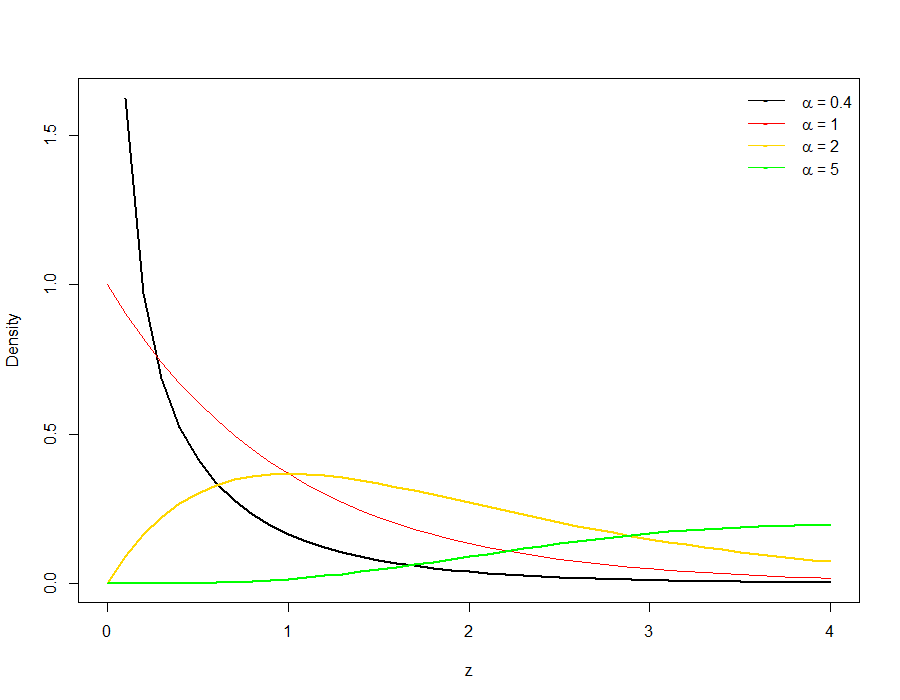
\includegraphics[ width=0.8\linewidth]{figures/gamma_distribution.png}
              \caption{Gamma density for different values at $\alpha$ when $\beta=1$.}
              \label{fig:gamma dist}
            \end{figure}
Figure \ref{fig:gamma dist} plots the shape of gamma p.d.f's for four values of $\alpha$.
When $\alpha = 1$ it is identical to the well know exponential distribution;
When $\alpha = 2$ we observe a more bell-shaped form.
The moment generating function of the gamma distribution is given as:


\begin{equation*}
     M_{Z}(t) = \frac{1}{(1 - \beta t)^\alpha}
\end{equation*}
Using the Laplace transform, we obtain:


\begin{equation}
     L_{Z}(t)  =  M_{Z}(-t) = \frac{1}{(1 + \beta t)^\alpha}
     \label{laplace population}
\end{equation}
It is common to assume that $ E[Z] = 1 $.
It then follows that $ \alpha \beta  = 1 $ and $ \alpha = 1 / \beta$.
Further we then have that $ V(Z) = \alpha \beta ^2 = \beta $.
Equation (\ref{laplace population}) then becomes:


\begin{equation}
     L_{Z}(t)  =  M_{Z}(-t) = \frac{1}{(1 + \beta t)^{1 / \beta}} = ( 1 + \beta t )^{-1 / \beta}
\end{equation}
Using (\ref{survival 1}), the survival function can now be written as:


\begin{equation}
   S(t) =  L_{Z}(A_{0}(t)) 
        = ( 1 + \beta A_{0}(t) )^{-1 / \beta} 
\end{equation}
Using (\ref{death intesity 1}), the population death intensity becomes:


\begin{equation}
     \mu(t) = \frac{1}{1 + \beta A_{0}(t)} \alpha_{0}(t)
     \label{deathIntensity population}
\end{equation}
This equation is useful because it gives a clear understanding of the effect of frailty on the death intensity of the population.
It becomes clear to observe from (\ref{deathIntensity population}) that when $\beta = 0 $ there is no frailty and $ \mu(t)$ and $\alpha_{0}(t)$ are identical.
We observe that when the frailty of the population decreases, the death intensity increase.
This can be observe in Figure \ref{fig:hazard and frailty} where we have chosen the basic rate $\alpha_{0}(t) = t^3$. We also observe that the population death intensity decreases with a strength determined by $\beta$.
%https://www.uio.no/studier/emner/matnat/math/STK4080/h16/undervisningsmateriell/lecture12_16.pdf


            \begin{figure}[tbh]
             \centering
              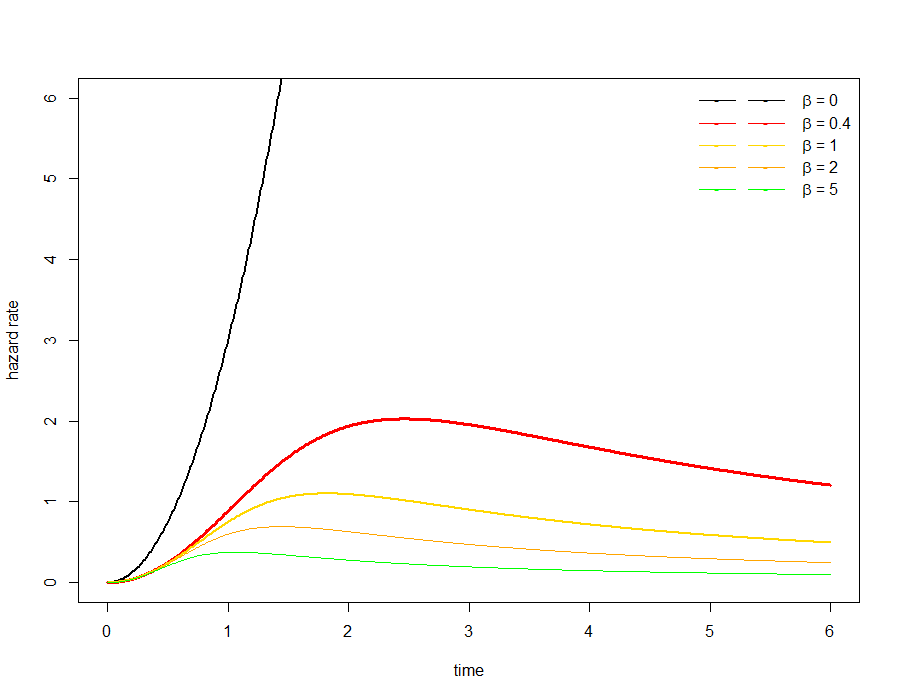
\includegraphics[ width=0.8\linewidth]{figures/hazard_frailty.png}
              \caption{Population hazard rates with various values of $\beta$}
              \label{fig:hazard and frailty}
            \end{figure}
            
         
         
\section{Two points frailty distribution}


An alternative to the gamma frailty model is a two-points model for the frailty.
Here we assume that the frailty $Z$ can take the two values $z_{1}$ and $z_{2}$ with probabilities $P(Z=z_{1}) = \pi_{1}$ and $ P(Z=z_{2}) = \pi_{2}$; ~~ $\pi_{1} + \pi_{2} = 1 $. \\
The Laplace transform becomes:
 
 
 \begin{equation}
     L_{Z}(t) = E[\exp(-t Z)] = \exp(-t z_{1}) \pi_{1} + \exp(-t z_{2}) \pi_{2}
 \end{equation}
The individual hazard can be written as :
 
 
\begin{equation}
    \alpha( t | Z) = Z \cdot\alpha_{0}(t)
    \label{frailty 1}
\end{equation}
With a two points frailty distribution we have two groups with respective death intensity, $z_{1}\alpha_{0}(t)$ and $z_{2}\alpha_{0}(t)$.
The population survival function is given by

\begin{equation}
  S(t)= L_{Z}(A_{0}(t))
        =\exp(-A_{0}(t) z_{1})\pi_{1} + \exp(-A_{0}(t) z_{2})\pi_{2}
    \label{survival_kap5}    
\end{equation}
In order to derive the population death intensity, we differentiate the survival function

\begin{equation}
\begin{split}
    S'(t) &= \exp(-A_{0}(t) z_{1})(-z_{1}\alpha_{0}(t))\pi_{1} +  \exp(-A_{0}(t) z_{2})(-z_{2}\alpha_{0}(t))\pi_{2} \\
        &= -[ \pi_{1}z_{1} \exp(-A_{0}(t)z_{1}) + \pi_{2}z_{2} \exp(-A_{0}(t)z_{2}) ]\cdot \alpha_{0}(t)
        \end{split}
\end{equation}
The population death intensity becomes :

 
\begin{equation}
 \begin{split}
      \mu(t)   &= - \frac{S'(t)}{S(t)} \\
               &= \frac{\pi_{1}z_{1} \exp(-A_{0}(t)z_{1})  + \pi_{2}z_{2} \exp(-A_{0}(t)z_{2})}{\pi_{1}\exp(-A_{0}(t)z_{1}) + \pi_{2}\exp(-A_{0}(t)z_{2}) } \cdot \alpha_{0}(t)\\
               &= W(t)z_{1}\alpha_{0}(t) + (1 - W(t))z_{2}\alpha_{0}(t)
    \label{deathIntensity population2}           
  \end{split}             
\end{equation}
where 


\begin{equation}
   W(t) = \frac{\pi_{1}\exp(-A_{0}(t)z_{1})}{\pi_{1}\exp(-A_{0}(t)z_{1}) + \pi_{2}\exp(-A_{0}(t)z_{2}) }
   \label{deathIntensity population3}
\end{equation}
Thus the population death intensity is a weighted average of the death intensities in the two groups.
The life expectancy up to age $a$ is :


\begin{equation}
    \begin{split}
     E[T_{a}] &= \int_{0}^{a} S(u)du \\
              &= \pi_{1}\int_{0}^{a} \exp(-A_{0}(u)z_{1})du +
                  \pi_{2}\int_{0}^{a} \exp(-A_{0}(u)z_{2})du
    \end{split} 
\end{equation}
If we introduce $ S_{0}(t) = \exp(-A_{0}(t)) $, we have 
\begin{equation*}
    \exp(-A_{0}(t)z_{i}) = S_{0}(t)^{z_{i}}
\end{equation*}
for $i = 1,2$.
Thus we obtain


\begin{equation}
    E[T_{a}]  =  \pi_{1}\int_{0}^{a} S_{0}(u)^{z_1}du + \pi_{2}\int_{0}^{a} S_{0}(u)^{z_2}du
    \label{life_expect_kapitel6}
\end{equation}



            



\section{Gompertz-Makeham}


We now assume a Gompertz-Makeham model for the basic hazard with parametrization

\begin{equation}
    \alpha_0(t) = a + ac^t = a + b\exp(t\log(c))
    \label{gompertz}
\end{equation}
where the constant $a$ can be interpreted as the risk of death from all causes which do not depend on age and the second element of the equation is the age-dependent component, which increases exponentially with age.
Then we have 


\begin{equation}
    \begin{split}
        A_{0}(t) &= \int_{0}^{t} \alpha_{0}(u)du \\
                 &= \int_{0}^{t} (a + b\exp(u\log(c)))du \\
                 &= \left[au + \frac{b}{\log(c)}\exp(u\log(c))\right]_0^t \\
                 &= at + \frac{b(\exp(t\log(c))-1)}{\log(c)}\\
                 &= at + \frac{b(c^t-1)}{\log(c)}
    \label{gompertz2}             
    \end{split}
\end{equation}
The corresponding survival function is:

\begin{equation}
    S_{0}(t) = \exp(-A_{0}(t)) = \exp( -at - \frac{b(c^t - 1)}{\log(c)})
\end{equation}
The population hazard may then be obtained from (\ref{deathIntensity population2}) and (\ref{deathIntensity population3}) using (\ref{gompertz}) and (\ref{gompertz2}) and the life expectancy up to age $a$ is given by (\ref{life_expect_kapitel6}).



%https://user.demogr.mpg.de/jwv/pdf/unobserved%20population%20heterogeneity.pdf




            \begin{figure}[tbh]
             \centering
              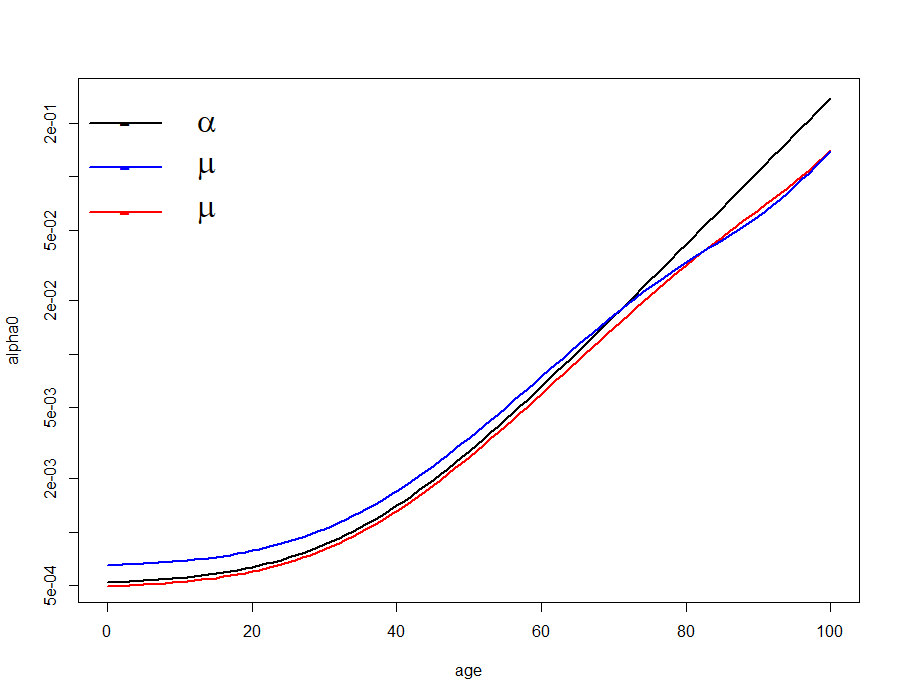
\includegraphics[ width=0.8\linewidth]{figures/Frailty_expect_lifelength.png}
              \caption{Basic hazard rate $\alpha_{0}(t)$ and population hazard rates $\mu (t)$ for the two points Gompertz-Makeham frailty distribution. See text for details}
              \label{fig:hazard and frailty_kap5}
            \end{figure}
Figure \ref{fig:hazard and frailty_kap5} shows the baseline death intensity $\alpha_{0}(t)$ of the Gompertz-Makeham form (black line) and the population hazards for a two-points frailty distribution when
$ a = 5*10^{-4} ;~b = 2*10^{-5 } ;~c = 1.10 $  and the probabilities are $\pi_{1}=0.7$ and $\pi_{2}=0.3$.The red line in Figure \ref{fig:hazard and frailty_kap5} is the population hazard when the frailty values are $z_{1} = 0.5$ and $z_{2} =2$.
We observe that the black and the red line overlap and are steadily increasing until the age of 70 years where $\mu$ (plot in red) starts slowing down.
The population life expectancy is here  83.95 years.
We then increase the value of the frailty $z_{2}$ from 2 to 3 while $z_{1}$ remains the same and we obtain a new population hazard $\mu(t)$ (plot in blue). 
We observe on the new plot of the population hazard that at younger ages the death intensity is higher than the basic hazard $\alpha_{0}(t)$ and also higher than the population hazard (plot in red) with the lower value of $z_{2}$. 
But from age 60 we observe a change of trend, the population hazard rate $\mu$ that had the highest mortality at the younger ages (blue line) increases less until age 80 where it cross the red line. With the new frailty value, the population life expectancy becomes 82.39 years.
That is the phenomena that was observed in chapter 4 where in Figures \ref{fig:CohortMortality 1910} - \ref{fig:CohortMortality 1950} the cohorts of Norwegian and Swedish women had a lower mortality at the younger ages than the women in Spain and Italy, but the opposite was the case for older ages.
We can conclude that the higher mortality observed in the population hazard $\mu(t)$ (plot in blue) for younger ages is the result of a higher number of individuals with a big value of frailty, since those individuals have a higher chance of dying than those with a smaller value of frailty. As the population get older, we have diminution of the number of frail individuals leading to the reduction of the mortality. That is why population hazard $\mu(t)$ (plot in blue), despite a higher mortality among the younger, has the lowest mortality among the older. 
In the next chapter, we will use the Gompertz-Makeham frailty distribution model to study the relationship between the period and the cohort mortality.


  
  
  
  
  
  




